%%-----------------------------------------------------------
%% 		DOCUMENT CLASS AND MARGIN DECLARATION		
\documentclass[a4paper, 11pt, twoside]{book}
\usepackage[top=4cm, bottom=4cm, left=3.5cm, right=3cm]{geometry}
%
%%-----------------------------------------------------------
%%-----------------------------------------------------------
%%		TEXT FORMATTING  & PAGE STYLE
\usepackage[english]{babel}
\usepackage[T1]{fontenc}
\usepackage[applemac]{inputenc}
\usepackage{enumerate}  
\usepackage{setspace}	%Setting the spaces between lines
\setstretch{1.0}
\usepackage{fancyhdr}
\pagestyle{fancy}
\fancyhead{}
\setlength{\headheight}{15pt}
\fancyhead[LE]{\nouppercase\leftmark}% LE -> Left part on Even pages
\fancyhead[RO]{\nouppercase\rightmark}% RO -> Right part on Odd pages
\fancyfoot[C]{\thepage}
\setlength{\parskip}{0pt}  %remove extra spaces between paragraphs
\newlength\tindent     %remove indent 
\setlength{\tindent}{\parindent}
\setlength{\parindent}{0pt}
\renewcommand{\indent}{\hspace*{\tindent}}
%%----------------------------------------------------------
%%----------------------------------------------------------
%%		TABLE & FIGURES
\usepackage{graphicx}
\usepackage{tabularx}
\usepackage{booktabs}
\usepackage{multirow}
\usepackage{float}
\usepackage[font=small,labelfont=bf,labelsep=period, tableposition=top,singlelinecheck=false]{caption}
%
%%-------------------------------------------------------
%%------------------------------------------------------
%%		MATH PACKAGES
\usepackage{amsmath}
\usepackage{amsxtra}
\usepackage{amstext}
\usepackage{amsthm}
\usepackage{amssymb}
\usepackage{amsfonts}
\usepackage{bm}
\usepackage{cancel}
\usepackage{siunitx}
%
%
\newcommand*{\bfrac}[2]{\genfrac{\lbrace}{\rbrace}{0pt}{}{#1}{#2}}
\DeclareMathOperator{\Imm}{Im}
\DeclareMathOperator{\Rea}{Re}
\DeclareMathOperator{\Tr}{Tr}
\DeclareMathOperator{\sign}{sgn}
%
%%---------------------------------------------
%%		BOX FOR EQUATIONS AND OTHER
\usepackage[leqno,fleqn,intlimits]{empheq}
\usepackage{fancybox}
\usepackage{color}
\definecolor{shadowcolor}{rgb}{0,.5,.5}
\setlength\shadowsize{2pt}
\usepackage[most]{tcolorbox}
\newtcolorbox[auto counter,number within=chapter]{mybox}[2][]{enhanced, breakable, width=\linewidth, sharp corners=all,  colback=white!95!black, ,fonttitle=\bfseries,
title=Box~\thetcbcounter: #2,#1}
%
%
\newtheorem{theorem}{Theorem}[section]
\newtheorem{corollary}{Corollary}[theorem]
\newtheorem{lemma}[theorem]{Lemma}
\newtheorem{Rule}{Rule}
%
%%-----------------------------------------------------
%%		NOTES
\usepackage[multiple]{footmisc}    %For multiple footnotes from the same source
\interfootnotelinepenalty=500000
%
%%Quote at the beginning of chapter
\makeatletter
\renewcommand{\@chapapp}{}% Not necessary...
\newenvironment{chapquote}[2][2em]
{\setlength{\@tempdima}{#1}%
\def\chapquote@author{#2}%
\parshape 1 \@tempdima \dimexpr\textwidth-2\@tempdima\relax\itshape}
 {\par\normalfont\hfill--\ \chapquote@author\hspace*{\@tempdima}\par\bigskip}
\makeatother
%%
%
%
%%----------------------------------------------------
%%       BIBLIOGRAPHY
%%\usepackage[super, square]{natbib}  %Super for superscripts and Square for square commas
%\usepackage{notoccite}
%%----------------------------------------------------------------------------------------
%%	LIST OF CONTENTS/FIGURES/TABLES PAGES
\setcounter{tocdepth}{2}  %1 to limit to section, 2 to subsection
\usepackage{color}   %May be necessary if you want to color links
\usepackage{hyperref}
\hypersetup{colorlinks=true,citecolor=black,linkcolor=black,linktocpage=true}
%%----------------------------------------------------------------------------------------

\begin{document}
\chapter*{Thermodynamics of PAH hydrogenation}

\section*{Introduction}
Let consider the following chemical equilibria for a \emph{polycyclic aromatic hydrocarbon} such as \emph{coronene}, $C_{24}H_{12}$:
\begin{gather}
    \text{C}_{24}\text{H}_{12+n} + H \rightarrow \text{C}_{24}\text{H}_{12+n+1} \nonumber \\
    2\text{H} \rightarrow \text{H}_2 \nonumber
\end{gather}
We define the \emph{fractional hydrogenation level} as
\begin{equation}
    f=\frac{N^0(H)}{N^0(H)/2+N^0(Co)} 
\end{equation}
where $N^0(H)$ is the total number of (extra) hydrogen available in a given sample and $N^0(Co)$ the total number of PAH molecules (bare \emph{plus} hydrogenated PAH molecules).
The free energy of $n$-fold hydrogenated structure is
\begin{equation}
    G_{n} = E_n - k_bT \ln{\mathcal{Z}^{int}_n}+k_bT\ln{\left(\frac{p_n}{\xi_n}\right)} \nonumber
\end{equation}
where $E_n$ is the DFT zero-point corrected energy, $\mathcal{Z}$ the internal partition function, $p_n$ the partial pressure and $\xi_n$ the thermal pressure, \emph{i.e.} $\xi_n=k_bT/\lambda_n^3$with $\lambda_n^3$ the \emph{De Broglie thermal wavelength}. The internal partition function accounting for rotational, vibrational and electronic contributions is given by
\begin{equation}
    \mathcal{Z}^{int}_{n} \simeq \frac{1}{\sigma_n}\left( \frac{T}{\theta}\right)^{3/2}\prod_{j=1}^{F_n}\left[1-\exp\left(-\frac{\hbar\omega_j^{(n)}}{k_bT}\right)\right]\mathcal{Z}_{n}^{el}  \label{eqapp:zint}
\end{equation}
where $\theta_n=\hbar^2/2I^{(n)}k_bT$ is the rotational temperature of the n-fold hydrogenated structure with $I^{(n)} = (\pi I^{(n)}_AI^{(n)}_BI^{(n)}_C)^{1/3}$ being its moment of inertia, given in terms of the principal values of inertia tensor, $\omega^{(n)}_j$ the normal mode frequencies ($j=1,2,...F_n$ where $F_n$ is the number of vibrational degrees of freedom, $F_n=3(36+n)-6$) and $\mathcal{Z}^{el}_n$ the electronic partition function, $\mathcal{Z}^{el}_n = 1+\mod(n,2)$.

For molecular hydrogen, the classical limit of rotational partition function is inappropriate at temperature $T \lesssim 100$ and one should consider the sum over \emph{all} states. To properly handle this situation, Equation \eqref{eqapp:zint} can still be employed, but in the following slightly modified form
\begin{equation}
    \mathcal{Z}^{int}_{H_2} \simeq \frac{1}{2}\frac{k_bT}{hcB}\left(1-\exp\left(-\frac{\hbar\omega}{k_bT}\right)\right)
\end{equation}
where the rotational constant $B$ can be adjusted in order to make the entropy, $S=-k_bT\ln{\mathcal{Z}}$, continuous at 298.15 K. The standard entropy $S$ can be computed from the \emph{Shomate equation}\footnote{
Shomate Equation for standard entropy $S^{\circ}$ (J/mol K) reads as
\begin{equation*}
S^{\circ} = A \ln{(t)} + Bt + C\frac{t^2}{2} + D\frac{t^3}{3} - \frac{E}{2t^2} + G
\end{equation*}
where $t=T/1000$ is the reduced temperature (K) and $A,B,C,D,E,G$ are temperature-dependent parameters (their values can be found in the NIST Chemistry WebBook.}.

\subsection*{Formation reaction energy: \texttt{phase diagram mode}}
If one is interested in determining the most stable species at a given thermodynamic condition, one may consider the "formation reaction"
\begin{equation}
    \text{C}_{24}\text{H}_{12} + \frac{n}{2}\text{H}_{2} \rightarrow \text{C}_{24}\text{H}_{12+n} \nonumber
\end{equation}
and the corresponding Gibbs free energy 
\begin{align}
    \Delta G_f(P,T,f^0) = G_n&(P,T)-G_0(P-p_{hy},T)+ \nonumber \\
     &-\frac{n}{2}G_{H_2}(p_{hy},T) \nonumber 
\end{align}
where $p_{hy}=f^0P$ and look, for given conditions, $P$, $T$ and $f^0$, for the smallest values. In \texttt{phase diagram mode}, the code computes such formation reaction energies in a prompted range of pressures, temperatures and fractional hydrogenation levels, and determine the most stable specie at any condition. 

\section*{Mixture free energy: \texttt{random walk mode}}
Let consider a mixture of PAH and (atomic/molecular) hydrogen and the problem of minimizing the mixture free energy. The initial mixture composition can be defined in terms of the number of molecules per each hydrogenated specie, $N^0_n$, plus the number of H atoms, $N^0_H$, and $\text{H}_2$ molecules, $N^0_{H_2}$. The associated initial Gibbs free energy is $G_{mix}^0$. The mixture composition can then be optimized \emph{stochastically}, by introducing random variations on each mixture components, simulating a sort of \emph{random walk} on the mixture composition. After any variation,  the mixture free energy, $G_{mix}^{1}$ is re-computed and compared with that of the previous step: if lower, $G_{mix}^1 < G_{mix}^0$, the newly random-generated composition is "saved" and used for the next step; otherwise that composition is "reject" and another random-generated composition is checked until $G_{mix}^1 < G_{mix}^0$ is found. Such stochastic procedure can be applied to a mixture with an initial composition consisting of only bare PAH molecules and an excess of $\text{H}_2$, \emph{i.e.} setting $N^0_i\simeq 0$ and $N^0_{H}\simeq 0$. In principle, one may introduce random variations on each $N_i$ from the very first optimization step. However, a more reasonable choice consists in allowing the $(i+1)$ structure to "form" in the mixture only once the mixture with the hydrogenated molecules up to $n=i$ has reached the equilibrium, thus better simulating the stepwise hydrogenation reaction\footnote{In other words, we are assuming that each hydrogenation step is "independent" of the others. Then, the equilibrium composition is reached through subsequent multiple "local" equilibria, $\text{C}_{24}\text{H}_{12+n} + \text{H} \rightarrow \text{C}_{24}\text{H}_{12+n+1}$.}. The following subsection briefly summarize the employed computational strategy.

\subsection*{Computational strategy}
The composition of a mixture at a give step $i$ is specified by a set $C=[N^{(i)}_{\text{H}}, N^{(i)}_{\text{H}_2}, $ $N^{(i)}_0, .., N^{(i)}_M]$, where $N^{(i)}_{\text{H}}$ is  the number of H atoms, $N^{(i)}_{\text{H}_2}$ is the number of $\text{H}_2$ molecules and $N^{(i)}_n$ that of $n$-hydrogenated PAH molecules, where $n=0,1,..M$ with $M$ the total number of hydrogenation steps (\emph{i.e.} $M=24$ for coronene)\footnote{Remind that this is the mixture with the optimized composition generated by the $i-1$ step.}. Variations on the abundances are introduced by adding to these, $\delta N^{(i)}_H$, $\delta N^{(i)}_{\text{H}_2}$, $\delta N^{(i)}_n$, that are given by (\emph{e.g.} for $N^{(i)}_n$)
\begin{equation}
dN^{(i)}_n = \frac{1}{W}2\left( \xi - \frac{1}{2} \right)N^{(i)}_n \label{eqapp:variations}
\end{equation}
where $\xi \in [ 0,1]$ is a (pseudo)-random number and $W$ is a scaling factor that allows tuning the extent of random variations (for $W=1$, $dN^{(i)}_n\in [ -N^{(i)}_n, N^{(i)}_n]$). Henceforth, we omit the superscript $i$. To ensure the mass balance of PAH molecules, we first set
\begin{gather*}
\tilde{N}_n = N_n + dN_n \\
\tilde{N}_t = \sum_n^M \tilde{N}_n
\end{gather*}
and then we properly re-define the random-variated populations at step $i$ as 
\begin{equation}
N'_n = \tilde{N}_n \frac{N^0_t}{\tilde{N}_t}
\end{equation}
where $N^0_t$ is the total number of PAH molecules that has been fixed at the outset. Once the abundance of H atoms in the mixture is modified (according to Equation \eqref{eqapp:variations}), the new population of $\text{H}_2$ molecules is given by the mass conservation law
\begin{equation}
dN_{\text{H}_2}  = \frac{1}{2} \left( -dN_{\text{H}} - \sum_n^M ndN'_n \right)
\end{equation}
Notice that $dN'_n \neq dN_n$ are the final "true" random-variation, \emph{i.e.} $dN'_n = N'_n - N_n$. With the newly random-generated mixture composition, the mixture Gibbs free energy is computed according to
\begin{equation}
    G_{mix}^{(i)} = \sum_{n=0}^MN'_nG_n+N'_{H}G_{H}+N'_{H_2}G_{H_2} \nonumber
\end{equation}

\begin{figure}
\centering
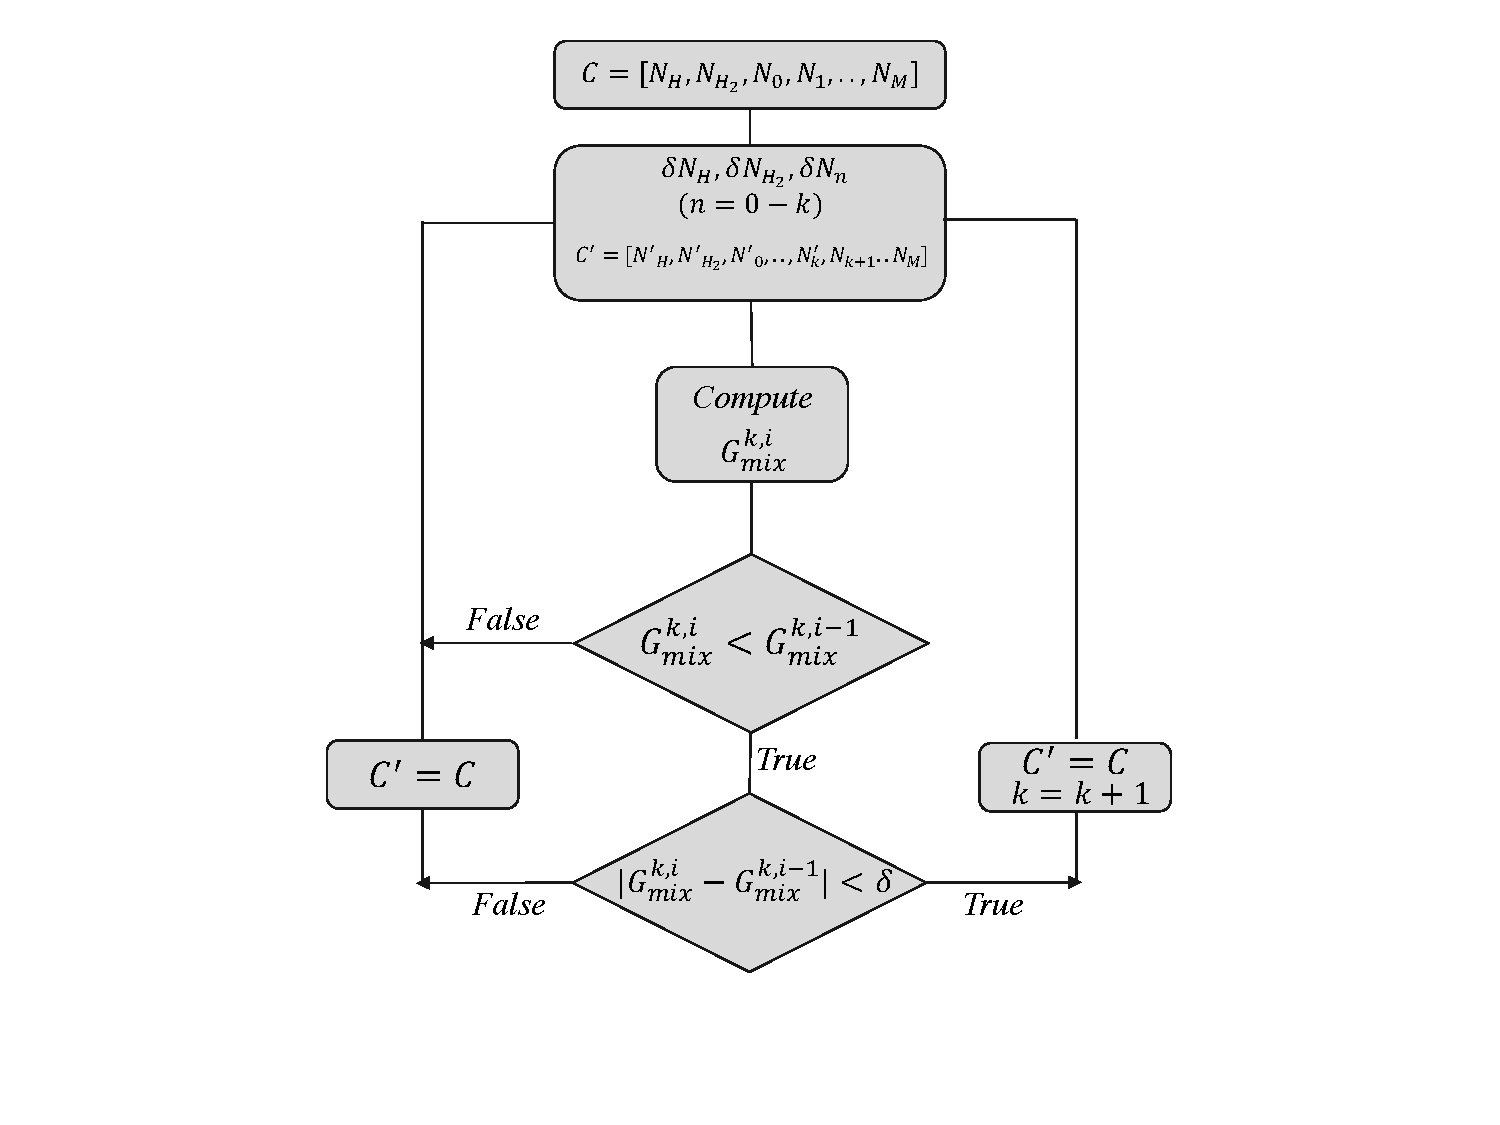
\includegraphics[width=0.68\textwidth]{flowchart}
\caption{A flowchart describing the optimization procedure.}
\label{fig:flowchart}
\end{figure}

As we mentioned before, we make the assumption of a stepwise optimization, where $[N_n, N_{n+1}, ..., N_{M}]$ populations are set to zero until $[N_{\text{H}}, N_{\text{H}_2}, N_0, ..., N_{n-1}]$ is optimized. In this sense, the full mixture composition optimization is divided into $M$ sub-optimizations, that we call $K=1, 2, ..., M$. The suboptimization $K=1$ involves the species $n=0,1$, $K=2$ the species $n=0,1,2$, etc. Since the interval of the random variation depends on the input composition at that step (see Equation \eqref{eqapp:variations}), at the very first step when the abundance of $N_n$ is "unconstrained", its value is set to a fraction (typically $1/100$ but this can be tuned in the input file) of the most abundant specie in the mixture at that moment. This choice should not affect the equilibrium just reached at the previous step. The flowchart in Figure \ref{fig:flowchart} summarize the optimization procedure.

At the end of any sub-optimization, the final equilibrium composition defined in terms of number of molecules ($N'_n$) is saved and written into a file called \texttt{\#\#-seqopt.out}. To make it "smooth", each of these mixture compositions are fitted according to:
\begin{equation}
    s(x)=\sum_{n=0}^{M} N'_n L_n(x) \nonumber 
\end{equation}
where $L_n(x)$ is a \emph{Lorentzian function}
\begin{equation}
    L_n(x) = \frac{1}{\pi}\frac{\frac{\gamma}{2}}{(x-n)^2+(\frac{\gamma}{2})^2} \nonumber
\end{equation}
and $\gamma$ is a scale parameter (the \emph{full width at half-maximum}) that allows tuning the shape of the Lorentzian. Lorentzian-fitted compositions are saved into files named \texttt{\#\#-lorentzian.out}


\end{document}


